\documentclass[noauthor,nooutcomes,12pt]{ximera}

\graphicspath{  
{./}
{./whoAreYou/}
{./drawingWithTheTurtle/}
{./bisectionMethod/}
{./circles/}
{./anglesAndRightTriangles/}
{./lawOfSines/}
{./lawOfCosines/}
{./plotter/}
{./staircases/}
{./pitch/}
{./qualityControl/}
{./symmetry/}
{./nGonBlock/}
}


%% page layout
\usepackage[cm,headings]{fullpage}
\raggedright
\setlength\headheight{13.6pt}


%% fonts
\usepackage{euler}

\usepackage{FiraMono}
\renewcommand\familydefault{\ttdefault} 
\usepackage[defaultmathsizes]{mathastext}
\usepackage[htt]{hyphenat}

\usepackage[T1]{fontenc}
\usepackage[scaled=1]{FiraSans}

%\usepackage{wedn}
\usepackage{pbsi} %% Answer font


\usepackage{cancel} %% strike through in pitch/pitch.tex


%% \usepackage{ulem} %% 
%% \renewcommand{\ULthickness}{2pt}% changes underline thickness

\tikzset{>=stealth}

\usepackage{adjustbox}

\setcounter{titlenumber}{-1}

%% journal style
\makeatletter
\newcommand\journalstyle{%
  \def\activitystyle{activity-chapter}
  \def\maketitle{%
    \addtocounter{titlenumber}{1}%
                {\flushleft\small\sffamily\bfseries\@pretitle\par\vspace{-1.5em}}%
                {\flushleft\LARGE\sffamily\bfseries\thetitlenumber\hspace{1em}\@title \par }%
                {\vskip .6em\noindent\textit\theabstract\setcounter{question}{0}\setcounter{sectiontitlenumber}{0}}%
                    \par\vspace{2em}
                    \phantomsection\addcontentsline{toc}{section}{\thetitlenumber\hspace{1em}\textbf{\@title}}%
                     }}
\makeatother



%% thm like environments
\let\question\relax
\let\endquestion\relax

\newtheoremstyle{QuestionStyle}{\topsep}{\topsep}%%% space between body and thm
		{}                      %%% Thm body font
		{}                              %%% Indent amount (empty = no indent)
		{\bfseries}            %%% Thm head font
		{)}                              %%% Punctuation after thm head
		{ }                           %%% Space after thm head
		{\thmnumber{#2}\thmnote{ \bfseries(#3)}}%%% Thm head spec
\theoremstyle{QuestionStyle}
\newtheorem{question}{}



\let\freeResponse\relax
\let\endfreeResponse\relax

%% \newtheoremstyle{ResponseStyle}{\topsep}{\topsep}%%% space between body and thm
%% 		{\wedn\bfseries}                      %%% Thm body font
%% 		{}                              %%% Indent amount (empty = no indent)
%% 		{\wedn\bfseries}            %%% Thm head font
%% 		{}                              %%% Punctuation after thm head
%% 		{3ex}                           %%% Space after thm head
%% 		{\underline{\underline{\thmname{#1}}}}%%% Thm head spec
%% \theoremstyle{ResponseStyle}

\usepackage[tikz]{mdframed}
\mdfdefinestyle{ResponseStyle}{leftmargin=1cm,linecolor=black,roundcorner=5pt,
, font=\bsifamily,}%font=\wedn\bfseries\upshape,}


\ifhandout
\NewEnviron{freeResponse}{}
\else
%\newtheorem{freeResponse}{Response:}
\newenvironment{freeResponse}{\begin{mdframed}[style=ResponseStyle]}{\end{mdframed}}
\fi



%% attempting to automate outcomes.

%% \newwrite\outcomefile
%%   \immediate\openout\outcomefile=\jobname.oc
%% \renewcommand{\outcome}[1]{\edef\theoutcomes{\theoutcomes #1~}%
%% \immediate\write\outcomefile{\unexpanded{\outcome}{#1}}}

%% \newcommand{\outcomelist}{\begin{itemize}\theoutcomes\end{itemize}}

%% \NewEnviron{listOutcomes}{\small\sffamily
%% After answering the following questions, students should be able to:
%% \begin{itemize}
%% \BODY
%% \end{itemize}
%% }
\usepackage[tikz]{mdframed}
\mdfdefinestyle{OutcomeStyle}{leftmargin=2cm,rightmargin=2cm,linecolor=black,roundcorner=5pt,
, font=\small\sffamily,}%font=\wedn\bfseries\upshape,}
\newenvironment{listOutcomes}{\begin{mdframed}[style=OutcomeStyle]After answering the following questions, students should be able to:\begin{itemize}}{\end{itemize}\end{mdframed}}



%% my commands

\newcommand{\snap}{{\bfseries\itshape\textsf{Snap!}}}
\newcommand{\flavor}{\link[\snap]{https://snap.berkeley.edu/}}
\newcommand{\mooculus}{\textsf{\textbf{MOOC}\textnormal{\textsf{ULUS}}}}


\usepackage{tkz-euclide}
\tikzstyle geometryDiagrams=[rounded corners=.5pt,ultra thick,color=black]
\colorlet{penColor}{black} % Color of a curve in a plot



\ifhandout\newcommand{\mynewpage}{\newpage}\else\newcommand{\mynewpage}{}\fi


\title{A gon block}
\author{Bart Snapp}

\begin{document}
\begin{abstract}
  We play with a new block.
\end{abstract}
\maketitle

\begin{listOutcomes}
\item Understand how to \textbf{use} the $n$-gon block.
\item Understand how the $n$-gon block \textbf{works}.
\item Demonstrate \textbf{competence} with the $n$-gon block.
\item Display both rotations and flips of regular $n$-gons using the
  $n$-gon block.
\end{listOutcomes}



The \mooculus\ Design company is at it again---and they need your
help. You see, someone designed a $n$-gon block for them:
\raisebox{-.4\height}{
\includegraphics{regularNGonBlockBLANK.png}}

The \mooculus\ Design company needs YOU to figure out how to USE the
block, explain how it WORKS on the inside, and DEMONSTRATE some
competency using it. 
\mynewpage



\begin{question}
  Let's figure out HOW to use
  \raisebox{-.4\height}{
\includegraphics{regularNGonBlockBLANK.png}}.
  \begin{enumerate}
  \item What happens when $n=5?$
  \item What happens when $n=-5?$
  \item What happens when $n=5$ and the block is PRECEDED by
    \raisebox{-.4\height}{
\includegraphics{turn72block.png}}?
  \end{enumerate}
  In each case, DESCRIBE what happens in WORDS and show off your work
  by displaying your SCRIPT and STAGE.
  \begin{hint}
    For the first two parts, use this SCRIPT:
    \begin{center}
      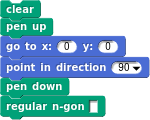
\includegraphics{nGonBlockClearBlank.png}
    \end{center}
  \end{hint}
  
  \begin{freeResponse}
    \begin{enumerate}
      \item When $n=5$, the block draws a regular pentagon with sides
        colored (clockwise from the top) yellow, green, blue, purple,
        red.  Here is my Script and my Stage:
        \begin{center}
          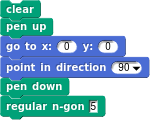
\includegraphics[width=.3\textwidth]{nGonPenBasicSCRIPT.png}   \qquad \fbox{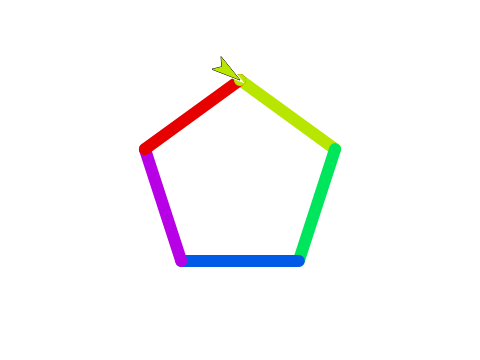
\includegraphics[width=.5\textwidth]{nGonPenBasicSTAGE.png}}
        \end{center}      
      \item When $n=-5$, the block draws a regular pentagon with sides
        colored (clockwise from the top) red, purple, blue, green,
        yellow.  Here is my Script and my Stage:
        \begin{center}
          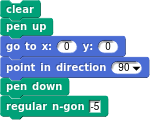
\includegraphics[width=.3\textwidth]{nGonPenFlipSCRIPT.png}   \qquad \fbox{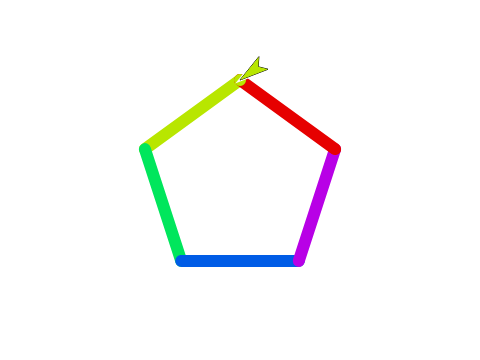
\includegraphics[width=.5\textwidth]{nGonPenFlipSTAGE.png}}
        \end{center}
      \item When $n=5$ and the block is PRECEDED by
        \raisebox{-.4\height}{
\includegraphics{turn72block.png}}, the
        block draws a regular pentagon with sides colored (clockwise
        from the top) red, yellow, green, blue, purple. Here is my
        Script and my Stage:
        \begin{center}
          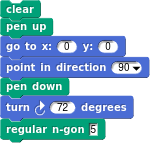
\includegraphics[width=.3\textwidth]{nGonPenRotSCRIPT.png}   \qquad \fbox{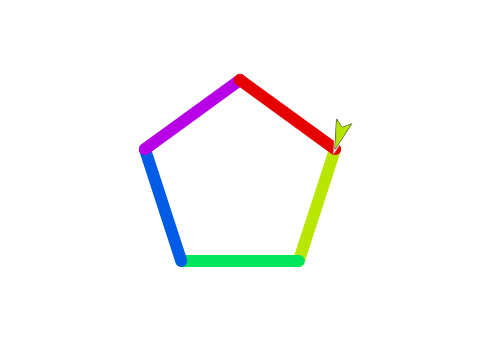
\includegraphics[width=.5\textwidth]{nGonPenRotSTAGE.png}}
        \end{center}  
    \end{enumerate}
  \end{freeResponse}
\end{question}
\mynewpage


\begin{question}
  How the n-gon block works.  Here's how it is coded:
  \begin{center}
    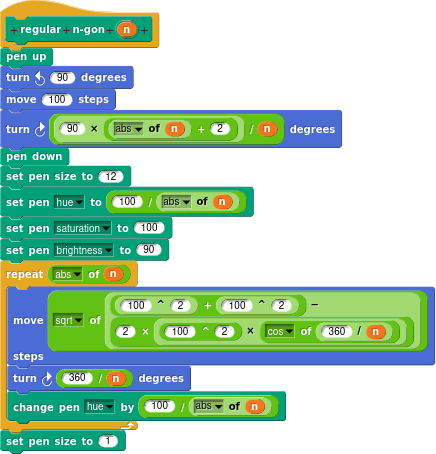
\includegraphics{regNGonBlockScript.png}
  \end{center}
  EXPLAIN how the script works, block-by-block as you would like to
  have it explained to you. \textbf{You may assume that $\boldsymbol n$ is positive in
  your explanation.} Use words, pictures, and so on, as needed/helpful
  in your explanation.
  \begin{freeResponse}
    This script does the following:
    \begin{enumerate}
    \item Turn the turtle $90^\circ$.
    \item Move $100$ units from the starting point.
    \item Then turn $180-\alpha$ degrees, where setting $\theta=
      360/n$:
      \begin{center}
        \begin{tikzpicture}[geometryDiagrams]
        \clip (-1,-1) rectangle (8,7);
        \coordinate (xmin) at (-6,0);
        \coordinate (xmax) at (6,0);
        \coordinate (ymin) at (0,-6);
        \coordinate (ymax) at (0,6);
        
        \tkzDrawSegment[->](xmin,xmax)
        \tkzDrawSegment[->](ymin,ymax)

        \coordinate (A) at (0,0);
        \coordinate (B) at (0,5);
        \coordinate (C) at (2.5,4.33);
        \coordinate (D) at (0,5.5);
        
        \tkzMarkAngle[black,thin,mark=](C,B,D)
        \tkzLabelAngle[pos=1.8](C,B,D){$180-\alpha$};

        %\tkzDrawSegment[black,line width=2pt](B,D)

        \tkzDrawSegment[black,line width=2pt](A,B)
        \tkzDrawSegment[black,line width=2pt](A,C)
        \tkzDrawSegment[black,line width=2pt](C,B)
        \tkzLabelSegment[black,right](A,C){$100$}
        \tkzLabelSegment[black,left](A,B){$100$}
        \tkzLabelSegment[black,above right](B,C){$\sqrt{100^2+100^2-2\cdot 100^2\cdot \cos(\theta)}$}
        
        \tkzMarkAngle[black,thin,size=.8cm](A,B,C)
        \tkzLabelAngle[pos=.5](B,C,A){$\alpha$};
        \tkzMarkAngle[black,thin,size=.8cm](B,C,A)
        \tkzLabelAngle[pos=.5](A,B,C){$\alpha$};
        \tkzDrawCircle[dashed](A,C)
        \tkzMarkAngle[black,thin,size=1.2cm,mark=](C,A,B)
        \tkzLabelAngle[pos=.9](C,A,B){$\theta$};
      \end{tikzpicture}
      \end{center}
      So
      \begin{align*}
        2\alpha + 360/n &= 180 \\
        2\alpha &=180 - 360/n\\
        2\alpha &=\frac{180n-360}{n}\\
        \alpha &= \frac{90n-180}{n}\\
        \alpha &= \frac{90(n-2)}{n}.
      \end{align*}
      So
      \begin{align*}
        180 - \alpha &= 180 - \frac{90(n-2)}{n}\\
        &= \frac{180n - 90n + 180}{n}\\
        &= \frac{90(n + 2)}{n}.
      \end{align*}
    \item We set the pen width to $12$ and the pen color to yellowish.
    \item Now we repeat the following steps $n$ times:
      \begin{enumerate}
      \item We use the Law of Cosines to find the side of the $n$-gon
        and travel that side.
      \item Turn $360/n$ degrees.
      \item Change the color by $n/100$.
      \end{enumerate}
    \item Finally we reset the pen size to $1$.
    \end{enumerate}
  \end{freeResponse}
\end{question}
\mynewpage



\begin{question}
  Use  \raisebox{-.4\height}{
\includegraphics{regularNGonBlockBLANK.png}} to draw this picture:
  \begin{center}
     \fbox{\includegraphics[width=.5\textwidth]{sevenGonBasicSTAGE.png}}
  \end{center}
  Show off your work by giving screenshots of your SCRIPT and STAGE as
  provided from \snap.
  \begin{freeResponse}
    Alright, so let's turn the regular $7$-gon by $5\cdot \frac{360}{7}\approx 257.14$ degrees, then draw the flip.
    \begin{center}
      \includegraphics[width=.3\textwidth]{sevenGonBasicSCRIPT.png}   \qquad \fbox{\includegraphics[width=.5\textwidth]{sevenGonBasicSTAGE.png}}
    \end{center}
    Perfect!
  \end{freeResponse}
\end{question}

\end{document}
